\documentclass{article}
\usepackage{amsmath, amsthm, amssymb, mathtools}
\usepackage{graphicx}
\newtheorem{theorem}{Theorem}
\newtheorem{proposition}{Proposition}
\def\R{\mathbb{R}}
\usepackage{xcolor}

\title{Differential invariant signatures for planar Lie group transformations of
images}
\date{\today}
\author{Huey, Duey, and Louey}

\begin{document}
\maketitle



% TODO
%   SRM: Kiwi picture to Richard, paste text from disappear.tex
%   RGB: Images for mesh, and for signatures

\section{Introduction}

A classic problem in image processing is to recognise the similarity or planar objects (point sets, curves, or images) up to transformations from a local planar group such as the Euclidean, similarity, and projective groups. Building on Cartan's solution to the equivalence problem, an influential new paradigm for this problem was introduced by Calabi et al. \cite{calabi98}, the differential invariant signature. The general theory has been developed extensively \cite{} and many examples computed for planar curves \cite{}, including the Euclidean, equi-affine, and projective groups. In this paper we develop and apply differential invariant signatures for planar images. Beyond merely computing the invariants, we emphasize the following.
\begin{enumerate}
\item We consider a very wide range of planar groups; the lattice structure of the set of groups influences
the relationship between the sets of invariants for the different groups.
\item We consider both finite-dimensional local Lie transformation groups and infinite-dimensional pseudogroups.
\item The signature must vary continuously with respect to the image, either for all smooth images or for all except
a set of sufficiently high codimension. This is essential if the signature is to be used to detect similarity of images, but it fails for the rational invariants found in the literature.
\item We do not insist that the signature is complete, i.e., that it  determines the image up to a transformation; for many applications an incomplete signature is sufficient. This may allow comparison of less smooth images.
\item We consider $k$-colour images for $k=1,2,\dots$. 
\item Putting these ingredients together, we arrive at a crucial ``meta-invariant'': the number of derivatives
of the image required as a function of the parameters (group, completeness, and number of colours).
\end{enumerate}

Let $G$ be a (finite or infinite-dimensional) local planar transformation group. 
A {\em $k$-colour image} is a triple $(f,\Omega,k)$ where $\Omega\subset\R^2$, $1\le k\in\mathbb{Z}$,
and $f\colon\Omega\to\R^k$. The function $f$ will be taken to be as smooth as necessary.
A transformation $\varphi\in G$ acts on images by $\varphi\cdot (f,\Omega,k) = (f\circ\varphi^{-1},\varphi(\Omega),k)$.
(As we work locally, we will usually omit the domain $\Omega$; if the number of colours $k$ is not given, we assume $k=1$.)  A differential invariant is an invariant of the prolonged action of $G$ on the derivatives of $f$, i.e., a function $I$ of the values of $f$ and its derivatives at a point such that $I(f)(x,y) = I(\varphi\cdot f)(\varphi(x,y))$. An {\em $m$-dimensional signature set} is the image of $m$ invariants $\mathcal{I}=(I_1,I_2,\dots,I_m)$, i.e. the
set $\mathcal{I}(f)(\Omega)\subset \mathbb{R}^m$. 
A signature set is complete for $f$ if it determines $f$ up to transformations from $G$, i.e. if $\mathcal{I}(\tilde f)(\tilde\Omega) = \mathcal{I}(f)(\Omega)$ implies there exists a transformation $\varphi\in G$ such that $\tilde f = \varphi\cdot f$ and $\tilde \Omega = \varphi(\Omega)$.

An algorithm to compute invariants and determine complete signature sets is described in \cite{olver2001}. First, the
entire set of invariants is computed using the method of moving frames. Second, determine the differential invariant order $s$ of $f$. Then the signature set of a maximal set of functionally independent invariants of order $s+1$ is complete. A third step is possible, in which the dimension of the signature set is reduced by eliminating those invariants whose values can be computed from the values of derivatives of some subset of the invariants. 

While we follow this approach in general, in specific cases we have computed invariants using other techniques
including the invariant tensor theorem and classical invariant theory. We shall see that this yields insights into the relationships between the different groups. We develop our approach through examples of progressively more complicated groups.

\subsection{Notation}
Let $G$ be a planar transformation group that acts on $k$-colour images $f
\colon \mathbb{R}^2 \rightarrow \mathbb{R}^k$ by $\varphi \cdot f \coloneqq
f \circ \varphi^{-1}$, where $\varphi \in G$.

When referring to coordinates, with $x \in \mathbb{R}^2$, we write $\hat{x}
= \varphi(x)$  and define the image post-transformation in the new
coordinates as
\begin{equation}
  \hat{f}(\hat{x}) = f(x).
\end{equation}
We derive relationships between the derivatives before and after
transformation by the chain rule:
\begin{equation*}
  f_{, i} = \hat{f}_{,k} \varphi_{k, i} 
\end{equation*}
etc. 


\begin{table}[h]
\begin{center}
\begin{tabular}{| l | c c c |}
\hline
\# derivs. & $k=1$ & $k=2$ & $k=3$ \\
\hline
SE(2) & 2 &1 & 1 \\
E(2) & 2 & 1 & 1 \\
Sim(2) & 2 & 1 & 1 \\
SA(2) & 2 & 2 & 2 \\
A(2) & 3 & 2 & 2 \\
$\mathrm{PSL}(2,\mathbb{C})$ & 3 & 3 & 3 \\
$\mathrm{PSL}(3,\R)$ & 3 & 2 & 2 \\
$\mathrm{Diff}_{\mathrm{vol}}$ & -- & 1 & 1 \\
$\mathrm{Diff}_{\mathrm{con}}$ & 3 & 1 & 1 \\
$\mathrm{Diff}$ & -- & -- & 0 \\
\hline
\end{tabular}
\caption{Number of derivatives of $f$ needed to construct a differential invariant signature of $f$ as a function of the group $G$ and the number of colours $k$ of $f$. The entry `--' indicates that there is no differential invariant signature in that case.}
\end{center}
\end{table}


\section{The Stamp Collection I: The Affine group and its subgroups}
In this section we consider all the groups whose transformation is of the
form. For these groups, the change of variables formulae are, in tensor,
and matrix notations,
\begin{align}
  f_{,i} &= \hat{f}_{, k} a_{ki} & \nabla f &= A^T \nabla \hat{f} \\
  f_{,ij} &= \hat{f}_{, kl} a_{ki} a_{lj} & 
  \nabla^2 f &= A^T \nabla^2 \hat{f} A
\end{align}
$\varphi(x) = Ax + b$ for some matrix $A$ and vector $b$.

\subsection{SE(2)}
In this case we have $A^TA = I$ and $\det A = 1$.

$E(2)$ is the Euclidean group of planar translations, rotations, and reflections.
We write $f_1 = \partial f/\partial x$ and $f_2 = \partial f/\partial y$ and use the summation convention, so that two well-known Euclidean invariants $\|\nabla f\|^2$ and $\nabla^2 f$ can be written as $f_i f_i$ and $f_{ii}$, respectively.

By the invariant tensor theorem (???ref???), all polynomial invariants of $f$ and its derivatives are the complete contractions. Up to order 2 there are 5 of these:
$ (f, f_i f_i, f_{ii}, f_{ij}f_i f_j, f_{ij}f_{ij})$
Any relation (syzygy) between 3 of these involves 2nd derivatives; so any derived relation involves 3rd derivatives and
cannot be used to determine a second order invariant. In this paper we shall focus on the signature sets
$ (f,f_i f_i,f_{ii})$
in $\mathbb{R}^3$
and
$(f, f_i f_i, f_{ii}, f_{ij}f_{ij})$
in $\mathbb{R}^4$. 
Although the first is not complete (we shall give an example of a parameterized family $(f_c,\Omega_c)$
of images, not related by Euclidean transformations, with the same signature sets), it can still
be used to distinguish {\em most} images.

\medskip

{\narrower\small

{\bf Aside 1. Testing the 3-dim signature.} Let $c$ be a parameter in the range $0<c<\pi/4$. Let $a = \sin(c)\cos(c)$ and $b=1/a$.
Consider the image $ f = a x y$ on domain $\Omega$ the sector  given in polar
coordinates by $\{(r,\theta)\colon 0 \le r \le b,\ 0 \le \theta \le c\}$.
Then in polar coordinates, the 3-dimensional signature set is
$$ (f, f_i f_i, f_{ii})(\Omega) = \{(ar^2 \sin\theta\cos\theta, a^2 r^2, 0)\colon 0 \le r \le b,\ 0 \le \theta \le c\}$$
which is the  triangle with vertices $(0,0,0)$, $(0,1,0)$, and $(1,1,0)$.
That is, all of these images (with different values of $c$) have the same signature set, but they are
not related by a Euclidean transformation.

}

\medskip

{\narrower\small 
{\bf Aside 2. Testing the 4-dim signature.} 
Now the 4-dimensional signature is checked. Let $(f,\Omega)$ be an image with
signature $\Sigma := \mathcal{I}(f)(\Omega) = (f,f_if_i,f_{ii},f_{ij}f_{ij})(\Omega)$. Let $(g,\widetilde\Omega)$ be
an image with the same signature set $\Sigma$. We need to determine coordinates 
$(\tilde x,\tilde y)$ on $\Sigma$ such that $\mathcal{I}(g)(x,y) = \mathcal{I}(f)(\tilde x,\tilde y)$.
The first component is $g(x,y)=f(\tilde x,\tilde y)$. That is, $g$ must be {\em some} coordinate
transformation of $f$. 
We seek the generators of solutions, setting $\tilde x = x + \varepsilon v^1(x,y)$,
$\tilde y = y + \varepsilon v^2(x,y)$. The first component yields $g_j = f_j + 2\varepsilon (f_i v^i v_j + 
f_{ij}v^i) + \dots$. This can be used to eliminate $g$ from the remaining equations, yielding

\begin{equation}
\begin{aligned}
f_i f_j v^{i}_j &= 0 \\
f_i v^i{jj} + 2 f_{ij}v^i_j&= 0\\
f_{jk}f_i v^i_{jk} + 2 f_{jk}f_{ik}v^i_j &= 0\\
\end{aligned}
\end{equation}

This is a set of 3 linear PDEs in $v^1$, $v^2$. Note that Euclidean
transformations have $v^i_j = -v^j_i$ and do satisfy all 3 equations. We can test
if the equations are locally overdetermined by differentiating and seeking compatibility 
conditions. We do this in Mathematica and find that differentiating the first equation 
3 times in $x$ and $y$, and the second two equations twice, yields a system
of 22 linear equations for the derivatives of $v^i$ at a point that,
for generic $f$, imply $v^i_{jk}=0$ at that point for all $i$, $j$, $k$. Since the point is arbitrary,
we conclude that the $v^i$ must be linear functions and that the transformation
is Euclidean.

}

\medskip

{\narrower\small 
{\bf Aside 3. Role of the invariants} 
All of the 2nd order differential invariants play known roles in geometric analysis:
\begin{enumerate}
\item $f_if_i=\|\nabla f\|^2$ is the Lagrangian density for the Laplacian;
\item $f_{ii}$ is the Laplacian, which plays a key role in Euclidean and conformal geometry;
\item $f_{ij}f_i f_j$ is the `infinity-Laplacian'; critical points of $\|\nabla f\|_{L^\infty}$ obey the PDE $f_{ij}f_i f_j=0$;
\item
$f_{ij}f_i f_j$ is also a Lagrangian density for $-2\det f_{ij}$, which arises in Monge--Amp\`ere equations and
which can be written in terms of the final 2nd order invariant as $-2 \det f_{ij} = f_{ij}f_{ij}-f_{ii}^2$.
\end{enumerate}
In addition, we shall see in later sections that functions of these invariants are invariants or
relative invariants for many groups that contain $E(2)$, namely $Sim(2)$, $SA(2)$, $A(2)$, $PSL(3,\mathbb{R})$, $PSL(2,\mathbb{C})$, and the conformal group.
}

\medskip

For $k$ colours, signature sets of dimension up to $k + k(k+1)/2$ can be 
chosen from the invariants $f^i$ and $f^i_m f^j_m$ for $i,j=1,\dots, k$.
For $k\ge 2$, first derivatives suffice. However, note that for
$k\ge 3$ the 3-dimensional signature $(f^1,f^2,f^3)$ 
is invariant under all local planar diffeomorphisms; a higher-dimensional
signature, involving first derivatives, is required.

The similarity group is the direct product of $E(2)$ with the positive scalings.
All invariants of $Sim(2)$ must be functions of invariants of its subgroup $E(2)$. We therefore
determine how the scalings $(x,y) \mapsto (\lambda x,\lambda y)$ transform the Euclidean invariants:
$$ (f, f_i f_i, f_{ii}, f_{ij}f_if_j, f_{ij}f_{ij}) \mapsto (f, \lambda^2 f_i f_i, \lambda^2 f_{ii}, \lambda^4 f_{ij}f_i f_j, 
\lambda^4 f_{ij}f_{ij}).$$
A standard approach in such a situation is to form rational invariants. One possibility is
$$\left(f, \frac{f_{ii}}{f_i f_i}, \frac{f_{ij}f_i f_j}{(f_i f_i)^2}, \frac{f_{ij}f_{ij}}{(f_i f_i)^2}\right).$$
However, this is singular at critical points of $f$. Critical points are a generic phenomenon of real
functions, so this invariant is not continuous for generic $f$.

Another possibility is
$$\left(f, \frac{(f_i f_i)^2}{f_{ij}f_{ij}}, \frac{(f_{ii})^2}{f_{ij}f_{ij}}, \frac{f_{ij}f_i f_j}{f_{ij}f_{ij}}\right).$$
This is singular only when $f_{ij}=0$ for all $i$ and $j$, a codimension 1 phenomenon for images.

However, an even better solution is possible, which also leads to a general technique for
dealing with rational invariants that we shall use throughout our study. 
Let $I_1=(f_i f_i)^2$, $I_2=(f_{ii})^2$, and $I_3=f_{ij}f_{ij}$. Then $I\mapsto \lambda^4 I$ under scalings.
Thus, positive rays in $I$ are similarity invariants. This leads to the invariant $I/\|I\|$ which
takes values in the unit sphere in $\mathbb{R}^3$. That is, it is an $S^2$-valued invariant.
It is singular only when $I=0$, i.e., when $f_i = f_{ij}=0$ for all $i$ and $j$, a codimension
3 phenomenon for images. Overall, we have the 3-dimensional Sim(2) signature set
$$(f,I/\|I\|)(\Omega)\subset \mathbb{R}\times S^2.$$
As any function of an invariant is also invariant, we can map the invariant into Euclidean space for convenience.
We can use, for example, the signature set $F(f)I/\|I\|(\Omega)\subset\mathbb{R}^3$ for some $F$.

Including $I_4=f_{ij}f_if_j$ in the set leads to an $\mathbb{R}\times S^3$-valued 4-dimensional signature set.

\medskip

{\narrower\small

{\bf Aside. Signatures with removable singularities.} As remarked above, at points
where $f_i=f_{ij}=0$ for all $i$, $j$, the $S^2$-valued signature () is not defined. However,
it is possible that for some images and some signatures, such singularities are removable.
Let $f$ be a cubic polynomial in $x$ and $y$ so that $f_i=f_{ij}=0$ at $(x,y)=(0,0)$.
Then the components of $((f_if_i)^2,(f_{ii})^2, f_{ij}f_{ij})$ are polynomials
of degree 8, 2, and 2 respectively. Therefore as $(x,y)\to(0,0)$ along a ray,
the $S^2$-valued signature $I/\|I\|$ tends to a point on the great circle with $I_1=0$. Along
different rays, it tends to different points. Thus the singularity at $(x,y)=(0,0)$ is not removable.

Now consider the slightly different signature set formed from 
$\tilde I = ((f_if_i)^2, f_{ij}f_{ij}, f_{ij}f_i f_j)$. 
Its components are polynomials of degree 8, 2, and 5, respectively, when $f$ is a cubic. Thus
as $(x,y)\to(0,0)$, the $S^2$-valued signature $\tilde I/\|\tilde I\|$ tends to
$(0,1,0)$ provided $f_{11}$, $f_{122}$, and $f_{22}$ are not simultaneously equal
to zero on a ray. But this happens if and only if the cubic $f$ is identically zero.
Therefore, this signature is continuous for arbitrary smooth functions
{\em except} those which obey $f_i = f_{ij}=f_{ijk}=0$ for some $(x,y)$,
which is a codimension 6 phenomenon for images.

}

\medskip

Although extremely simple and apparently tied to scaling symmetries, this trick has
wide applicability. As is well known, for many group actions orbits cannot be separated by continuous
invariants. In contrast, generic orbits of rational algebraic groups are always separated by
a finite set of rational invariants \cite{hubert}. Suppose we have found some rational
invariants of images for some group that can be written in the form
$$ \left( \frac{N_1}{D},\dots,\frac{N_r}{D}\right)$$
where the $N_i$ are continuous rational functions (not necessarily polynomials), and $D$ is a polynomial.
Then we have
$$ \varphi \cdot \left(D,N_1,\dots,N_r\right) \mapsto \psi(\varphi)(D,N_1,\dots,N_r)$$
---that is, essentially a scaling. There are now two cases.

Case 1. $\psi(\varphi)>0$ for all $\varphi\in G$. In this case we have an $S^r$-valued invariant that
is continuous except where $D=N_1=\dots N_r=0$. When $r\ge 2$, this is typically a codimension
1 condition for images. That is,  $r$ rational invariants with the same denominator yield $r$ continuous
invariants.

Case 2. $\psi(\varphi)$ takes on both signs. (As the action is continuous, this case is only
possible if $G$ is not connected.) In this case we have an invariant on the projective space $\mathbb{R}P^r$. The options are to work directly on this space or to map it into a Euclidean space, by an embedding or immersion
(e.g. $\mathbb{R}P^2$ can be embedded in $\mathbb{R}^4$ or immersed in $\mathbb{R}^3$).

The crucial requirement is that at least two invariants share the same denominator. In all
of the examples in this paper, only one denominator arises.

If $r$ is large enough it is possible to increase the codimension of the bad set of images without
increasing the dimension of the signature. For example, if $r=3$ we can project
$ (D, N_1, N_2^2+N_3^2)$
to $S^2$; this is only singular when $D=N_1=N_2=N_3=0$, which is typically a codimension-2 situation for images.

\section{Equi-affine and affine planar curves}

We illustrate the usefulness of this technique by reconsidering the example of equi-affine signature curves
of planar curves studied in Calabi et al. \cite{calabi}. Here $r\colon S^1\to\R^2$ is a planar curve, on 
which the equi-affine group acts by $(A,b)\cdot r = A r + b$, $\det A = 1$. The signature curve
of \cite{calabi} is $(\kappa,\kappa_s)$ where $\kappa$ is equi-affine curvature and $\kappa_s$
is derivative with respect to equi-affine arclength. It is sufficient for our purposes to record
this in local coordinates in which the curve is written $y=u(x)$:
$$\kappa = \frac{3 u_2 u_4 - 5 u_3^2}{9 u_2^{8/3}}$$
$$\kappa_s  \frac{9 u_2^2 u_5 - 45 u_2 u_3 u_4 + 40 u_3^3}{27 u_2^4}$$
Here $u_n = d^n u/dx^n$.
It is remarked in \cite{calabi}  that ``affine geometry requires the (unfortunate) restriction to convex curves'',
as the curvature and its derivatives are not defined when $u_{xx}=0$, e.g. at inflection points; in \cite{calabi} 
it is suggested to deal with this by studying the asymptotic behaviour of the signature curve as it blows
up near inflection points. 

We now show that using a spherical instead of a planar signature curve, with singularities removed,
yields a signature curve that is continuous for all planar curves with inflection points of any finite order.

Let
$$ I = (u_2^8, u_2^8(9\kappa)^3, u_2^4 (27\kappa_s)^2) = (u_2^8, (-5 u_3^2 + 3 u_2 u_4)^3,(9 u_2^2 u_5 - 45 u_2 u_3 u_4 + 40 u_3^3)^2).$$
The equiaffine group acts on $I$ as $(A,b)\cdot I = A_{11}^{-24}I$, so projection 
to the sphere yields an equiaffine signature curve. If $u\sim x^n$ as $x\to 0$ with $n\ge 3$, then
$I\sim(x^{8(n-2)}, x^{6(n-3)},x^{6(n-3)})$ as $x\to 0$. Therefore the signature curve
tends to a well-defined point on $I_1=0$ as $x\to 0$ for an inflection point
of any order $n$, and the signature is continuous except for a set of 
curves of infinite codimension.

(Note that the precise behaviour of the signature near singularities is important. A signature
that behaved like $(x^3, x^3, x)$ as $x\to 0$ would not yield a continuous $S^2$-valued signature,
as it tends to $(0,0,1)$ as $x\to 0^+$ and to $(0,0,-1)$ as $x\to 0^-$; removing the sign requires an extra step.)

In this example, the projection technique is more or less equivalent to
Calabi et al.'s suggestion of analyzing the blowup of the planar signature. 

The same technique provides a continuous affine signature. The next equi-affine invariant is
$$ \kappa_{ss} = \frac{-160 u_{3}^4 + 255 u_2 u_3^2 u_4 - 45 u_2^2 u_4^2 - 63 u_2^2 u_3 u_5 + 9 u_2^3 u_6}{27 u_2^({16/3}}.$$
Under the action of the affine group, we
have
$$(\kappa,\kappa_s,\kappa_{ss})\mapsto (\lambda^{-4/3},\lambda^{-2},\lambda^{-8/3})$$
where $\lambda = \det A$. Therefore we form the rational relative invariant of weight $-8$
$$\tilde I = (\kappa^6,\kappa_s^4,\kappa_{ss}^3).$$
Projection to the sphere provides an $S^2$-valued 4th order affine signature curve.
The denominator of each term is $u_{xx}^{16}$. If $u\sim x^n$ as $x\to 0$ with 
$n\ge 3$, then $\tilde I \sim (x^{-4(n+1)},x^{-4(n+1)},x^{-4(n+1)})$.
Therefore the signature curve tends to a well-defined point on $S^2$ as $x\to 0$ 
for an inflection point of any order $n$, and, as for the equiaffine case, the signature is continuous except for
a set of curves of infinite codimension.

\section{Special affine group {\bf SA(2)}}

The special or equi-affine group $SA(2)$ is the group of transformations $\mathbf{x}\mapsto A\mathbf{x}+\mathbf{b}$
where $\det A =1$.  This case leads to an intriguing connection with classical invariant theory \cite{olverclassical}.
This is because the derivatives of $f$ transform as
\begin{equation}
\begin{aligned}
f_i & \mapsto A_{ij} f_j \\
f_{ij} & \mapsto A_{il} A_{jm} f_{lm}\\
f_{ijk} & \mapsto A_{il}A_{jm}A_{kn}f_{lmn}\\
\end{aligned}
\end{equation}
and so on. These are the same transformation rules obey by a linear, quadratic, and cubic binary forms.
The Taylor series of $f$ {\em is} the sum of a constant, a linear binary form, a quadratic binary form, and so on.
 In this case we have a vector
space $V=\R^2$, the space $V_n$ of binary forms of degree $n$ ($\cong Sym(V^{\otimes n})$), and seek
joint invariants of $V_1\oplus V_2\oplus V_3\oplus\dots$ under the action of $SL(V)$. The ones we need,
the joint invariants of $V_1\oplus V_2\oplus V_3$, 
were found first by Alexander Bessel in 1869 \cite{bessel}. (See page 108 of \cite{draisma}.)

The invariants can all be written as ``transvectants''. 
Given forms $g$ and $h$, their $p$th transvectant $(g,h)_p$ is given by (up to a constant)
$$ (g,h)_p = \sum_{i=0}^p (-1)^p {p \choose i} 
\frac{\partial^p g}{\partial x^{p-i}\partial y^{i}}
\frac{\partial^p h}{\partial x^{i}\partial y^{p-i}}
$$
If $g$ is degree $m$ and $h$ is degree $n$ then $(g,h)_p$ is degree $m+n-2p$; transvectants of degree 0 are invariants.
The general method to find them is to first compute how many invariants there are of each degree (this can be done independently), form the available invariants from transvectants, and then finding an independent set -- this is done by evaluating the derivatives of a candidate set on random forms and checking if they have full rank.  

Let $\ell$ be the linear form $f_i x_i$ and $q$ be the quadratic form $f_{ij} x_i x_j$.
For derivatives up to 2nd order, we need the invariants of $V_1\oplus V_2$. 
The polynomial invariants are generated by
$$(q,q)_2 = \det f'' =: C$$
and
$$(q,\ell^2)_2 = f_{22}f_1^2 + f_{11}f_2^2 - 2 f_{122} f_1 f_2 =: D.$$
The group orbits on $V_1\oplus V_2$ are codimension 2 and generic orbits are separated by these invariants.

In fact, it is easy to see directly that these two quantities are invariant. Switching to matrix notation, we 
have $f'' \mapsto A f'' A^T$ so that $\det f'' \mapsto \det(A)\det(f'')\det(A^T) = \det(f'')$,
and $(f')^T (f'')^{-1} f' \mapsto (A f')^T A^{-T} (f'')^{-1} A^{-1}  (A f') = (f')^T (f'')^{-1} f'$. 
The product of these two invariants is $(f')^T \mathrm{adj}(f'') f' = D$.

This quantity $D$ turns out to be of interest in its own right; we discuss aspects and interpretations of it here.
\begin{enumerate}
\item $D$ can of course be written as a function
of the invariants of its Euclidean subgroup, namely
$$D = f_{ii} f_j f_j - f_{ij}f_i f_j.$$
\item
$D$ has a more directly Euclidean interpretation in terms of the curvature $\kappa$ of the level sets of $f$:
$$ D = \kappa (f_i f_i)^{3/2}$$
(This follows from the expression $\kappa = \nabla\cdot n$, where $n=\nabla f/\|\nabla f\|$ is the 
unit normal to the level sets of $f$; see Section \ref{sec:}.)
\item
$D$ is directly related to the equiaffine arclength. This is $d\mu = \kappa^{1/3}ds$, where
$\kappa$ is Euclidean curvature and $ds$ is Euclidean arclength. Therefore,
$$ D = \kappa \|\nabla f\|^3 = \left(\frac{d\mu}{ds}\|\nabla f\|\right)^3.$$
The normal and tangent directions to the level sets of $f$ are at right angles
to each other. If, under an equiaffine transformation, the distance
between level sets scales by $\lambda$, then $\nabla f$ scales by $1/\lambda$, 
and $ds$ also scales by $1/\lambda$ as the transformation is area preserving.
Thus the right hand side of () is equiaffine invariant.
\item We shall show in Section \ref{sec:proj} that $D$ is also relative invariant of the projective group.
\item The 2nd order invariants () imply that any equiaffine-invariant 2nd order PDE can be written in the form
$\mathcal{F}(f, C, D)=0$.
The special case of equations of the form $\mathcal{F}(f,C)=0$, namely Monge--Amp\`ere equations, is well known.
Naturally occurring examples of $\mathcal{F}(f,C,D)=0$ would be of great interest.
\item $D$ is an $SA(2)$-invariant Lagrangian density for $C$:
$$ \delta\int \left(f_{22}f_1^2 + f_{11}f_2^2 - 2 f_{122} f_1 f_2\right) \, dx\, dy = - 6\det f_{ij}.$$
\end{enumerate}

For derivatives up to 3rd order, we need the invariants of $V_1\oplus V_2\oplus V_3$, which are
given by those given above together with new ones containing 3rd derivatives. As there are 4 independent
entries in $f'''$, and the group parameters have already all been taken out, there should be at least 4 new invariants. It turns out that to generate all the polynomial invariants requires not 4 but 13 new polynomial invariants.
Of these, 2, 4, 4, 2, and 1 have degree 3, 4, 5, 6, and 7 respectively \cite{draisma}.
A set of generating invariants for $V_1\oplus V_2\oplus V_3$ is given in Table \ref{tab:sl2},
where  $c$ is the cubic form $f_{ijk}x_i x_j x_k$. 

To summarize, for 1-colour images, the 3-dimensional signature $(f,C,D)$ requires 2 derivatives;
a 4-dimensional signature requires 3 derivatives. Such a signature is given by 
$(f,C,D)$ together with one of the invariants containing $c$ in Table \ref{tab:sl2}, 
such as $I_6$ (which is linear in $f'''$) or $I_3$ (which does not contain $\ell$, so it
does not vanish at critical points.)


\begin{table}
\label{tab:sl2}
\begin{center}
\begin{tabular}{| l | l | l | l |}
\hline
name & deg & weight & invariant \\
\hline
$I_1$ & 2 & 4 & $(q,q)_2$\\
& & & $\quad \propto C := \det f_{ij}$ \\
$I_2$ & 3 & 4 & $(q,\ell^2)_2$\\
& & & $\quad  \propto D := f_{11}f_2^2 + f_{22} f_1^2 - 2 f_{12} f_1 f_2$ \\
$I_3$ & 3 & 8 & $(q,(c,c)_2)_2$\\
& & & $\quad  \propto  f_{22} f_{112}^2 + f_{11} f_{122}^2 + f_{12} f_{111}f_{222} $ \\
& & & $\qquad- f_{22}f_{111}f_{122}
- f_{12} f_{112}f_{122} -f_{11} f_{112} f_{222}$\\
$I_4$ & 3 & 6 & $(c,q\ell)_3$\\
& & & $\quad   \propto f_2 f_{22} f_{111} - 2 f_2 f_{122} f_{112} - f_1 f_{22} f_{112} $\\
& & & $\qquad + f_2 f_{11} f_{122}
+ 2 f_1 f_{122} f_{122} - f_1 f_{11} f_{222}$\\
$I_5$ & 4 & 12 & $((c,c)_2,(c,c)_2)_2$ \\
$I_{6}$ & 4& 6 &  $(c,\ell^3)_3$\\
& & & $\quad \propto E := f_{111} f_2^3 - 3 f_{112}f_1 f_2^2  + 3f_{122} f_1^2 f_2  - f_{222}f_1^3 $\\
$I_{7}$ &4 & 8 &  $((c,c)_2,\ell^2)_2$\\
$I_{8}$ & 4& 8 &  $(c \ell,q^2)_4$\\
$I_{9}$ & 5& 12 &  $(c^2,q^3)_6$\\
$I_{10}$ &5 &8  &  $(((c,\ell)_1,q)_1,\ell^2)_2$\\
$I_{11}$ &5 &12 &  $(q,(((c,c)_2,c)_1,\ell)_1)_2$\\
$I_{12}$ &5 & 10 &  $(((c,c)_2,q)_1,\ell^2)_2$\\
$I_{13}$ & 6& 12&  $(\ell c,(\ell c,\ell c)_2)_4$\\
$I_{14}$ & 6& 14&  $(((c,c)_2,q)_1,(q \ell,c)_2)_2$\\
$I_{15}$ & 7& 18 &  $(q^3,c((c,c)_2,c)_1)_6$\\
\hline
\end{tabular}
\end{center}
\end{table}



For more colours,  we are seeking invariants of $k V_1 \oplus k V_2 \oplus \dots$. One can take transvectants of any components of $f$ to get invariants.

For $k=2$ colours, there is only one  invariant formed from 1st derivatives, namely $((f^1)',(f^2)')_1 = f^1_1 f^2_2 - f^1_2 f^2_1$ (the Poisson bracket $\{f^1,f^2\}$). So again two derivatives are necessary, even for 
a 3-dimensional signature.

 For $k\ge 3$ colours, a new phenomenon enters.  There are plenty of invariants
formed from 1st derivatives, namely $\nabla f^i \times \nabla f^j$ for $i<j$. But these are all invariant under the bigger group $\mathrm{Diff}_{\mathrm{vol}}$ of local volume preserving diffeomorphisms. So the Poisson brackets
cannot form a complete invariant for $SA(2)$. Two derivatives are always needed no matter how many
colours we have. The relation $SA(2)\subset \mathrm{Diff}_{\mathrm{vol}}$ acts an obstruction
to $SA(2)$, an instance of the phenomenon of hidden symmetry.


\subsection{Invariants, hey!}
literature (Cartan, Olver, Russians, Draisma), motivation, etc,

\subsection{Invariants for images}
Colour and the lack of independence. Fractal dimension 

Calculating derivatives (discussion on desirability thereof).
Euclidean-invariant smoothing is a thing, other groups not so much.

\subsection{Introducing the cast}
Define each group, mesh image of what transformations can look like

\subsection{Technical wank}
Completeness, degeneracy, moving frames as concept table of numbers of
derivatives, all that jazz, maybe scaling technique
for dealing with invariants of non-unit weight


\section{The invariants}
One subsection for each group. Mathematical details/theorem/derivation, no
examples
\subsection{SA(2), E(2), SE(2), and Sim(2), or some better title}
\begin{theorem}
  SA(2) invariants up to second order are:
  I0, I1, I2 from Jupyter document
\end{theorem}

Corollary for E(2), SE(2), R2 and Sim(2)

Commentary on geometric interpretation of these things.
\subsection{A(2)}
\begin{theorem}
  General affine invariants using transvectants
\end{theorem}
Relative invariants and weights go here? probably

The affine group of transformations  $\mathbf{x}\mapsto A\mathbf{x}+\mathbf{b}$, $\det A\ne 0$,
is common in image processing. It is the product of $SA(2)$ with the positive scalings, thus
we can use the same method as for $Sim(2)$ to construct invariants. Each $SA(2)$ invariant
becomes a relative invariant of $A(2)$ of a certain weight, given in Table \ref{tab:sl2}.
 As $C$ and $D$ have weight 4 and
$E$ has weight 6, a simple 3-dimensional signature set is formed from $f$ together with
the weight-12 relative invariant
$$(C^3,D^3,E^2)$$
projected to $S^2$. This signature is continuous except at points where $C=D=E=0$, which 
is a codimension 1 phenomenon for images; the bad points include $f_1=f_2=\det f_{ij}=0$.

As for $Sim(2)$, signature sets which are continuous on sets of higher codimension can be
formed by including more (relative) invariants.

First consider including {\em all 15} invariants of Table \ref{tab:sl2}. They define
a map $I\colon \mathbb{R}^9\to \mathbb{R}^{15}$ where 
$(f_i,f_{ij},f_{ijk})$ are the 9 coordinates on the domain. As $\dim SL(2,\mathbb{R})=3$, 
the rank of this map is at most 6. Indeed, the rank is 6 at generic points, and
most level sets of $I$ are 3-dimensional.
However, $I^{-1}(0)$ is not 3-, but 5-dimensional. 
Despite the high degree of the equations $I=0$ (the product of the individual
degrees, more than 2 billion), the equations can be reduced to a single quadratic.
One component of $I^{-1}(0)$ can be written
$$ \begin{pmatrix}f_1 \\f_2 \\f_{11} \\f_{12} \\f_{22} \\f_{111} \\f_{112} \\f_{122} \\f_{222}\end{pmatrix}=
\alpha_3^{-2}\begin{pmatrix}\alpha_1\alpha_3\\
 \alpha_1\alpha_3(\alpha_2-\beta)\\ 
 \alpha_3\alpha_4\\
\alpha_3\alpha_4(\alpha_2-\beta)\\
\alpha_4(2\alpha_2^2-2\alpha_2\beta - \alpha_3\alpha_5)\\
\alpha_3\\
\alpha_2\\
\alpha_5\\
2\beta^3 + \alpha_2(3\alpha_3\alpha_5 - 2\alpha_2^2)
\end{pmatrix}$$
where $\beta=\sqrt{\alpha_2^2-\alpha_3\alpha_5}$ and
$\alpha_1,\dots,\alpha_5$ are parameters.
That is, the level set $I^{-1}(0)$ contains a union of several orbits of $SA(2)$ and these
cannot be distinguished using the entire set of relative invariants.

Likewise, we can consider the reduced set $\widetilde I := (I_1,I_2,I_3,I_4)$. 
We find that the highest dimensional component of $\widetilde{I}^{-1}(0)$ 
again has dimension 5. (It includes, but is not idential to, $I^{-1}(0)$.) 
So the 4-dimensional signature formed from $f$ and $\widetilde I$
is continuous except on a set of images of codimension $5-2=3$, the same 
as  the 15-dimensional signature formed from $f$ and $I$. 
Many other reduced sets (maps from $\widetilde{I}$ to $\R^4$ have the same property
and can be used instead.

The root cause of the obstruction to finding a signature that is continuous on a set of images
of codimension greater than 3 is that rational invariants are only guaranteed
to separate generic orbits, not all orbits. Characterizing the orbits
that can be separated by rational invariants a question that
has to be tackled separately in each case.

Thus for 1-colour images, an affine signature set or 3 or 4 dimensions requires three derivatives.


With $k\ge 2$ colours, there are plenty of available invariants formed from  two derivatives, already 9 when $k=2$. 
However, as with $SA(2)$, we can never get away with one derivative because all the 1-derivative invariants,
such as $\{f^1,f^2\}/\{f^1,f^3\}$ 
are also invariant
under $\mathrm{Diff}_{\mathrm{vol}}$ (even though $A(2)$ is not even a subgroup of $\mathrm{Diff}_{\mathrm{vo}l}$).


\subsection{M\"obius and Projective (finite dimensional)}
\begin{theorem}
  Moving frame invariants for M\"obius
\end{theorem}

The M\"obius group $\mathrm{PSL}(2,\mathbb{C})$ acts on the Riemann sphere
$\overline{\mathbb{C}} = \mathbb{C}\cup\infty$ by 
$$ \phi\colon \overline{\mathbb{C}} \to \overline{\mathbb{C}},\quad \phi(z) = \frac{\alpha z + \beta}{\gamma z + \delta},\quad \alpha,\beta,\gamma,\delta\in\mathbb{C}, \quad
\alpha\delta-\beta\gamma\ne 0.$$
Identifying $\R^2$ with $\mathbb{C}$, the M\"obius group is a real 6-dimensional local Lie group acting on $\mathbb{R}^2$.
It is the smallest nonlinear planar group that contains $SE(2)$, and it is the set of biholomorphic maps of the Riemann sphere; it also has direct applications in image processing since it arises in the {\em conformal camera} model of vision, in which scenes are projected radially onto a sphere \cite{lenz1990group,turski2004geometric,turski2005geometric}. 
Different shapes may be related by M\"obius transformations, as is explored by
Petukhov \cite{petukhov1989non} for biological objects: in one example, the human skull grows approximately by M\"obius transformations.  Note also that Thompson \cite{thompson1942growth} famously deformed images of one species to match those of another, many of his examples using conformal mappings, and thus may be approximated (or even determined by) M\"obius transformations. Discussing this work, Milnor \cite{milnor2010growth}  argued that ``The geometrically simplest way to change the relative size of different body parts would be by a conformal transformation. It seems plausible that this simplest solution will often be the most efficient, so that natural selection tend to choose it.'' (Milnor was thinking of 3D conformal transformations, whose restriction to 2D is the M\"obius transformations.)

The M\"obius action is locally identical to the full conformal group up to and including second order. Therefore, there are no new M\"obius invariants, apart from the conformal invariants, up to second order. At third order, there are no new group parameters
to be eliminated; we therefore expect four independent invariants, of which two are the conformal invariants found in the previous section. We find the two remaining independent invariants using the moving frame method.

The 0th order moving frame translates $z$ to
$\beta$. We can therefore take $\beta=0$; we are also free to take $\delta=1$. This leaves 4 group parameters $a,b,c,d$, where $\alpha = a + i b$, $\gamma = c + i d$,
to be determined as follows. First we prolong the action to 3rd derivatives of $f$. There are 9 derivatives of
$f$ of order 1, 2, and 3, so there must be at least 5 invariants.

The prolonged action is
\begin{equation}
\small
\arraycolsep=1.4pt
\left(
\begin{array}{c}
  \bar f_1 \\ \bar f_2 \\ \bar f_{11} \\ \bar f_{122} \\ \bar f_{22} \\ \bar f_{111} \\ \bar f_{112} \\ \bar f_{122} \\ \bar f_{222} 
 \end{array}
 \right)
 = 
\left(
\begin{array}{ccccccccc}
 a & b & 0 & 0 & 0 & 0 & 0 & 0 & 0 \\
 -b & a & 0 & 0 & 0 & 0 & 0 & 0 & 0 \\
 2\mu & -2 \rho & a^2 & 2 a b & b^2 & 0 & 0 & 0 & 0 \\
 2 \rho & 2\mu & -a b & a^2\!-b^2 & a b & 0 & 0 & 0 & 0 \\
 -2\mu & 2 \rho & b^2 & -2 a b & a^2 & 0 & 0 & 0 & 0 \\
 -6 (2 b c d+a \lambda) & 6 (2 a c d-b\lambda) & 6 a \mu &
  M_{64}  & -6 b \rho & a^3 & 3 a^2 b & 3 a b^2 & b^3 \\
 -6 (2 a c d-b\lambda) & -6 (2 b c d+a \lambda) & M_{73}& M_{74} & 
 M_{75} & -a^2 b & a^3\!-2 a b^2 & 2
   a^2 b\!-b^3 & a b^2 \\
 6 (2 b c d+a \lambda) & -6 (2 a c d-b\lambda) & M_{83} & M_{84} & M_{85} & a b^2 & b^3\!-2
   a^2 b & a^3\!-2 a b^2 & a^2 b \\
 6 (2 a c d-b\lambda) & 6 (2 b c d+a \lambda) & 6 b \mu & 
  M_{94} & 6 a \rho & -b^3 & 3 a b^2 & -3 a^2 b & a^3 \\
\end{array}
\right)\left(
\begin{array}{c}
f_1 \\ f_2 \\ f_{11} \\ f_{122} \\ f_{22} \\ f_{111} \\ f_{112} \\ f_{122} \\ f_{222} 
 \end{array}
 \right).
 \end{equation}
 where
 \begin{equation*}
 \small
 \begin{array}{lll}
M_{64}=-12abc+6d(a^2-b^2), & 
M_{73}=4 d a^2+6 b c a-2 b^2 d, & 
M_{74}=-6 c a^2+12 b d a+6 b^2 c, \\
 M_{75}=-2 d a^2-6 b c a+4 b^2 d, &
 M_{83}=2 c a^2-6 b d a-4 b^2 c, &
 M_{84}=6 (d a^2+2 b c a-b^2 d),\\
 M_{85}=-4 c a^2+6 b d a+2 b^2 c,& 
 M_{94}= -12a b d + 6c(a^2-b^2),\\
\lambda=d^2-c^2, & 
\mu = b d - a c, & 
\rho = b c + a d.
\end{array}
\end{equation*}

The moving frame calculation now proceeds as follows.
\begin{enumerate}
\item The frame $\bar f_1=1$, $\bar f_2=0$ determines the group parameters
$$ a = f_1/(f_i f_i),\quad b = f_2/(f_i f_i).$$

\item The frame $\bar f_{122}=\bar f_{22}=0$ determines the group parameters
$$ c = (2 f_1f_2f_{122} - f_{11}f_2^2 - f_{22}f_1^2)/(2 f_i f_i)^2$$
$$ d = (f_{122}f_1^2 - f_1 f_2 f_{11} - f_{122}f_2^2 - f_{22} f_1 f_2)/(2 f_i f_i)^2.$$

\item The 2nd order invariant is then given by $\bar f_{11}$ using (); it is 
$$\bar f_{11} = \frac{f_ii}{f_i f_i},$$
which we have already determined as the conformal invariant $J_2/J_1$.

\item The four 3rd order invariants are then given by $\bar f_{111},\dots,f_{222}$ using (). They are
rational functions with numerators of degree 6 and denominators $(f_i f_i)^4$. We call
the numerators $K_1,\dots, K_4$; they are relative invariants of weight 8.
\end{enumerate}

It is clear that there must be 2 syzygies between the relative invariants $J_1,\dots,J_4,K_1,\dots,K_4$.
They are easily found algebraically to be
$$K_2 = -K_4 + J_1 J_4$$
and
$$K_3=-K_1 +J_1 J_3 + 2 J_1^2 J_2^2.$$
Therefore we can take $K_1$ and $K_4$ as two independent M\"obius invariants. They are
$K_1=
f_2 ^5 f_{222} + \frac{9}{2} f_2 ^2 f_{22}^2 f_1 ^2 + 
 f_2 ^3 f_{222} f_1 ^2 + \frac{3}{2} f_{22}^2 f_1 ^4 - 
 9 f_2 ^3 f_{22} f_1  f_{12} + 
 3 f_2  f_{22} f_1 ^3 f_{12} + \frac{3}{2} f_2 ^4 f_{12}^2 - 
 9 f_2 ^2 f_1 ^2 f_{12}^2 + \frac{3}{2} f_1 ^4 f_{12}^2 + 
 3 f_2 ^4 f_1  f_{122} + 3 f_2 ^2 f_1 ^3 f_{122} + 
 3 f_2 ^4 f_{22} f_{11} + 3 f_{22} f_1 ^4 f_{11} + 
 3 f_2 ^3 f_1  f_{12} f_{11} - 
 9 f_2  f_1 ^3 f_{12} f_{11} + \frac{3}{2} f_2 ^4 f_{11}^2 + 
 \frac{9}{2} f_2 ^2 f_1 ^2 f_{11}^2 + 3 f_2 ^3 f_1 ^2 f_{112} + 
 3 f_2  f_1 ^4 f_{112} + f_2 ^2 f_1 ^3 f_{111} + 
 f_1 ^5 f_{111}, 
 $
 
 $K_4=-3 f_2  f_{22}^2 f_1 ^3 + 
 f_2 ^2 f_{222} f_1 ^3 + f_{222} f_1 ^5 + 
 9 f_2 ^2 f_{22} f_1 ^2 f_{12} - 
 3 f_{22} f_1 ^4 f_{12} - 6 f_2 ^3 f_1  f_{12}^2 + 
 6 f_2  f_1 ^3 f_{12}^2 - 3 f_2 ^3 f_1 ^2 f_{122} - 
 3 f_2  f_1 ^4 f_{122} - 3 f_2 ^3 f_{22} f_1  f_{11} + 
 3 f_2  f_{22} f_1 ^3 f_{11} + 3 f_2 ^4 f_{12} f_{11} - 
 9 f_2 ^2 f_1 ^2 f_{12} f_{11} + 
 3 f_2 ^3 f_1  f_{11}^2 + 3 f_2 ^4 f_1  f_{112} + 
 3 f_2 ^2 f_1 ^3 f_{112} - f_2 ^5 f_{111} - 
 f_2 ^3 f_1 ^2 f_{111}
$


In previous work \cite{mobius}, two independent 3rd order M\"obius invariants were calculated
from the classical M\"obius geometry of curves. Namely, the M\"obius arclength 
of a curve is $\sqrt{|\kappa_s|}ds$, were $ds$ is Euclidean arclength. Under any conformal map $\phi$,
both $ds$ and $1/\|\nabla f\|$ scale by $|\phi'|$. The sign of $\kappa_s$ is also  invariant,
hence $\kappa_s/\|\nabla f\|^2$ is  invariant for any invariant curve. Calculating this invariant
for the level sets of $f$ and for their orthogonal curves yields two invariants of $f$ that
we call $\lambda_t$ and $\lambda_n$, respectively. Writing 
them out in full and comparing to the invariants founds above shows that they are related very simply, by

$$ \frac{K_2}{\|\nabla f\|^8} = \lambda_t$$
$$\frac{K_4}{\|\nabla f\|^8} =\lambda_n$$

We do not know of any equivalent characterization of the invariants $K_1$, $K_3$ in
terms of classical M\"obius geometry.

We now have that
$$ (J_1^4, J_2^4, J_1 J_3, J_1 J_4, K_1, K_4)$$
are 6 relative invariants of weight 8. Projecting any subset to a sphere provides a M\"obius signature.
For example, the image $f$ together with the projection of $(J_1^4, J_2^4, K_1)$ provides a 3-dimensional signature.
Any such signature that includes $J_1$ and $J_2$ is singular when $f_1=f_2=f_{ii}=0$, a codimension 1
phenomenon for images. 

For images with $k\ge 2$ colours, recall that M\"obius and conformal transformations cannot be distinguished
by their action on second derivatives. Therefore at least 3 derivatives are needed, no matter how many 
colours we have. We can use, for example, the invariants arising from the curvature of the level sets of
each colour. Replacing the first relative invariant $\|\nabla f\|^2$ by $\sum_{j=1}^k \|\nabla f^j\|^2$,
and the second relative invariant $f_{ii}$ by $\sum_{j=1}^k (f^j_{ii})^2$, increases
the codimension of the singular images from 1 to $3k-2$.

\section{{\bf $\mathbf{PSL}({\bf 3},\R)$}}

We consider the 8-dimensional group $\mathrm{PSL}(3,\R)$ acting on $\R^2$ by projective transformations, i.e.,
$$(x,y) \mapsto \left(\frac{a x + b y + j}{l + g x + h y}, \frac{c x + d y + k}{l+ g x + h y}\right).$$
We will construct invariants using the moving frame method. The 0th order moving frame translates $(x,y)$ to
$(0,0)$. We can therefore take $j=k=0$; we will also take $l=1$. This leaves 6 group parameters $(a,b,c,d,g,h)$
to be determined as follows. First we prolong the action to 3rd derivatives of $f$. There are 9 derivatives of
$f$ of order 1, 2, and 3, so there must be at least 3 invariants.

The prolonged action is
\begin{equation}
\tiny
\arraycolsep=1.4pt
\label{eq:prolong}
\left(
\begin{array}{c}
  \bar f_1 \\ \bar f_2 \\ \bar f_{11} \\ \bar f_{122} \\ \bar f_{22} \\ \bar f_{111} \\ \bar f_{112} \\ \bar f_{122} \\ \bar f_{222} 
 \end{array}
 \right)
 = 
\left(
\begin{array}{ccccccccc}
 a & c & 0 & 0 & 0 & 0 & 0 & 0 & 0 \\
 b & d & 0 & 0 & 0 & 0 & 0 & 0 & 0 \\
 -2 a g & -2 c g & a^2 & 2 a c & c^2 & 0 & 0 & 0 & 0 \\
 -b g-a h & -d g-c h & a b & b c+a d & c d & 0 & 0 & 0 & 0 \\
 -2 b h & -2 d h & b^2 & 2 b d & d^2 & 0 & 0 & 0 & 0 \\
 6 a g^2 & 6 c g^2 & -6 a^2 g & -12 a c g & -6 c^2 g & a^3 & 3 a^2 c & 3 a c^2 & c^3 \\
 2 g (b g+2 a h) & 2 g (d g+2 c h) & -2 a (2 b g+a h) & -4 (b c g+a d g+a c h) & -2 c (2 d
   g+c h) & a^2 b & a (2 b c+a d) & c (b c+2 a d) & c^2 d \\
 2 h (2 b g+a h) & 2 h (2 d g+c h) & -2 b (b g+2 a h) & -4 (b d g+b c h+a d h) & -2 d (d g+2
   c h) & a b^2 & b (b c+2 a d) & d (2 b c+a d) & c d^2 \\
 6 b h^2 & 6 d h^2 & -6 b^2 h & -12 b d h & -6 d^2 h & b^3 & 3 b^2 d & 3 b d^2 & d^3 \\
\end{array}
\right)\left(
\begin{array}{c}
f_1 \\ f_2 \\ f_{11} \\ f_{122} \\ f_{22} \\ f_{111} \\ f_{112} \\ f_{122} \\ f_{222} 
 \end{array}
 \right).
 \end{equation}

First, recall from the analysis of the subgroup $A(2)$ that under $f\mapsto f\circ \phi$, $\phi\in A(2)$, we have 
\begin{equation}
\label{eq:D}
D \mapsto (\det \phi')^2 D\circ \phi
\end{equation}
where $D = f_{1}^2 f_{22} + f_2^2 f_{11} - 2 f_1 f_2 f_{122}$. 
A direct calculation using (\ref{eq:prolong}) shows that the same transformation rule (\ref{eq:D}) holds for $\phi\in\mathrm{PSL}(3,\R)$.
That is, $D$ is a relative invariant of weight 2 of this action. From (\ref{eq:D}), the sign of $D$ is invariant and therefore
the choice of moving frame must depend on the sign of $D$.

\begin{enumerate}
\item The frame $\bar f_1 = 1$  determines the group parameter $$a = (1-c f_2)/f_1.$$
\item The frame $\bar f_2=  0$ determines the group parameter $$b = -d f_2/f_1.$$
\item Substituting this choice of $a$ and $b$ and examining the dependencies of $f_{11}$, $f_{122}$, $f_{22}$, and $f_{222}$ on the remaining group parameters allows them to be solved sequentially, as follows.
\item We have $\bar f_{22} = d^2 D/f_1^2$; therefore if $D>0$ we choose the frame
$\bar f_{22} = 1$ and $$d = f_1/D^{1/2}.$$
\item The frame $\bar f_{222} = 0$ determines the group parameter
$$ h = \frac{d(f_{222}f_1^3 - 3 f_1^2 f_2 f_{122} + 3 f_1 f_2^2 f_{112} - f_2^3 f_{111})}{6 f_1 D}.$$
\item The frame $\bar f_{122}=0$ determines the group parameter
$$ c = \frac{h f_1^2}{d D} - \frac{f_1 f_{12} - f_2 f_{11}}{D}.$$
\item The frame $\bar f_{11}=0$ determines the group parameter
$$ g = \frac{1}{2 f_1^2}(f_{11} + 2 c ( f_1 f_{12} - f_2 f_{11} ) + c^2 D).$$
\end{enumerate}

Having determined the frame, any function of the remaining derivatives $\bar f_{111}$, $\bar f_{112}$, and $\bar f_{222}$,
as given in (\ref{eq:prolong}),
provides invariants. We choose
$$ (f_{111}, f_{112}^2, f_{122})=\left(\frac{J_1}{D^6},\frac{J_2}{D^9},\frac{J_3}{D^3}\right)$$
because these all have denominators given by integer powers  of $D$, resolving the issue caused
by the sign of $D$. Therefore,
$$ (D^{18}, J_1^3, J_2^2, J_3^6)$$
are all relative invariants of weight 36; so projecting any subset of them of them to a sphere
yields a 3rd order invariant signature.

However, these signatures can be simplified and made more robust, as follows.

The components of $J$ are polynomials of degree 16, 24, and 8, respectively, and are extremely complicated when written out explicitly. More seriously, $J$ vanishes on generic images. This can be seen as follows. 
Recall the $SA(2)$ invariant $E$ defined in (\ref{eq:E}).
%Let
%$$ E := f_{222}f_1^3 - 3 f_{122}f_1 f_2^2 + 3 f_{112}f_1^2 f_2 - f_{111}f_2^3$$
Then the components of $J$ have the structure
$$ J_1 = E^4 + D P_{13},\quad J_2 = (E^3 + D P_9)^2,\quad J_3=E^2 -12 D P_5$$
where the $P_n$ are polynomials of degree $n$. Therefore $J=0$ when $D=E=0$, which 
is a codimension 0 phenomenon for images. In particular, $D=E=0$ at critical points.

The structure of () suggests considering the combination $J_1 - J_3^2$ which turns out to obey
$$J_1 - J_3^2 = 144 D^4 P_4.$$
Therefore, as $J_1/D^6$ and $J_3/D^3$ are invariant, so is $P_4/D^2$. 
Moreover, {\em the numerator of this new invariant does not vanish at critical points.} 
It has the structure
$$P_4 = -4(\det f_{ij})^2 + Q_4,$$
where $Q_4$ is a polynomial of degree 4 that vanishes when $f_1=f_2=0$. In conclusion, the
relative invariant of weight 12
$$ (D^6, P_4^3, (E^2-12D P_5)^2)$$
can be projected to $S^2$ yielding a projective invariant of images that
is singular only when $D=E=P_4=0$, which is a codimension 1 phenomenon for images.
(One can check that $D=E=0\nRightarrow P_4=0$.) In particular, at critical points it tends to
$$ (0, (2\det f_{ij})^6, 0)$$
and hence critical points with $\det f_{ij}\ne 0$ have signature $(0,1,0)$.

For completeness we write out the invariants explicitly:

$Q_4=4 f_1  f_{12} ^2 f_{122}  - 
f_1 ^2 f_{122} ^2 - 
 2 f_{222}  f_1  f_{12}  f_{11}  + 
 2 f_{22}  f_1  f_{122}  f_{11}  - 
 6 f_{2}  f_{12}  f_{122}  f_{11}  + 
 2 f_{2}  f_{222}  f_{11} ^2 + 
 f_{222}  f_1 ^2 f_{112}  - 
 6 f_{22}  f_1  f_{12}  f_{112}  + 
 4 f_{2}  f_{12} ^2 f_{112}  + 
 f_{2}  f_1  f_{122}  f_{112}  + 
 2 f_{2}  f_{22}  f_{11}  f_{112}  - 
 f_{2} ^2 f_{112} ^2 + 
 2 f_{22} ^2 f_1  f_{111}  - 
 f_{2}  f_{222}  f_1  f_{111}  - 
 2 f_{2}  f_{22}  f_{12}  f_{111}  + f_{2} ^2 f_{122}  f_{111} $
 
$P_5=f_{222}  f_{1} ^3 f_{12}  - 
f_{22}  f_{1} ^2 f_{12} ^2 + 
 2 f_{2}  f_{1}  f_{12} ^3 - 
 f_{22}  f_{1} ^3 f_{122}  - 
 f_{2}  f_{1} ^2 f_{12}  f_{122}  + 
 f_{22} ^2 f_{1} ^2 f_{11}  - 
 f_{2}  f_{222}  f_{1} ^2 f_{11}  - 
 2 f_{2}  f_{22}  f_{1}  f_{12}  f_{11}  - 
 f_{2} ^2 f_{12} ^2 f_{11}  + 
 2 f_{2} ^2 f_{1}  f_{122}  f_{11}  + 
 f_{2} ^2 f_{22}  f_{11} ^2 + 
 2 f_{2}  f_{22}  f_{1} ^2 f_{112}  - 
 f_{2} ^2 f_{1}  f_{12}  f_{112}  - 
 f_{2} ^3 f_{11}  f_{112}  - 
 f_{2} ^2 f_{22}  f_{1}  f_{111}  + 
 f_{2} ^3 f_{12}  f_{111} $
 
 Including $J_2$ in addition provides a 4-dimensional signature set, but does not increase
 the codimension of the set of bad images.
 
Further invariants can be found by noting that, for any planar transformation group and any two invariants
$I^1$ and $I^2$, $\nabla I^1 \times \nabla I^2$ is a relative invariant of weight 1; that is,
$$\nabla I^1 \times \nabla I^2\mapsto (\det \phi')(\nabla I^1 \times \nabla I^2).$$
Applying this operation to $f$ and the 4 3rd order invariants yields $5\cdot4/2=1$0  4th order invariants.

{\color{red}Following needs work:}

For $2$-colour images, there are 3  second order relative invariants of weight 2,
namely $(D_1,D_2,(\nabla f^1\times \nabla f^2)^2)$. Together with $(f^1,f^2)$, these yield
a 4-dimensional $\mathbb{R}^2\times S^2$-valued signature using only 2nd derivatives.
With $k>2$ colours there are many more 2nd order invariants; however, as the action
of the projective group on 1st derivatives is indistinguishable from that of the full
diffeomorphism group, it is not possible to have a 1st order signature that distinguishes
projectively-related images from diffeomorphically-related ones.


\begin{theorem}
  Moving frame invariants for Projective
\end{theorem}

\subsection{Infinite dimensional diff groups (diff con, diff vol, diff)}

The conformal
group is infinite-dimensional, but still small enough that images have local differential invariants.

We first compute the invariants of the conformal group up to 3rd order. Instead of applying the method
of moving frames, we perform a direct calculation using the defining geometric properties of the conformal
group.

The conformal transformations are defined to be those that preserve angles. At first order, the only
available data are $(f,f_i)$, which do not create any angles. There are no first order invariants.

At second order, we first consider the action of conformal maps on the Euclidean invariants
$f_i f_i$ and $f_{ii}$.

Let $\psi := \varphi^{-1}$. For any diffeomorphism, the derivatives of $f$ transform as
$$f_i \mapsto f_j \psi^j_i$$
and
$$f_{ij} \mapsto f_{kl} \psi^k_i\psi^l_j + f_{k}\psi^k_{ij}.$$
Therefore the Laplacian of $f$ transforms as
$$ f_{ii} \mapsto f_{kl} \psi^k_i \psi^l_i + f_k \psi^k_{ii}.$$
When $\psi=u + i v$ is conformal, $\psi_{k,ii}=0$ because the components of conformal maps are harmonic functions,
and the Cauchy-Riemann equations give $\psi_{k,i}\psi_{l,i} = (u_x^2 + u_y^2)\delta_{kl}$. Therefore,
$$ f_{ii} \mapsto f_{ii}(u_x^2+u_y^2).$$
Here $u_x^2+u_y^2=\det\psi^k_i$ is the local scaling factor of the transformation.
Note also that
$$f_i f_i \mapsto f_k f_l \psi_{k,i} \psi_{l,i} = f_k f_k (u_x^2 + u_y^2).$$
That is, $f_{ii}$ and $f_i f_i$ are both relative invariants of weight 2.

Therefore, $f_{ii}/(f_i f_i)$ is a conformal invariant. By itself, it is not useful for images as it is singular at critical points of $f$.

At higher order,  representing $\psi(z) = a_0 + a_1 z + a_2 z^2 + \dots$ where $z=x+iy$ and $a_i\in \mathbb{C}$ shows that
2 real group parameters, $Re(a_n)$ and $Im(a_n)$, enter at order $n$. There are $n+1$ independent derivatives of $f$ of order $n$, 
so there must be at least $n-1$ independent invariants of order $n$. For $n=2$, we have we have found the single invariant above.

The transformation of 1st derivatives is more clearly written in complex variables as
$$ f_x + i f_y \mapsto a_1 (f_x + i f_y).$$
Given any two real invariants $g,h$, the real and imaginary parts of $(g_x+i g_y)(h_x-i h_y)$ are
relative invariants of weight 2. This generates the required two invariants of order 3. (We have
repeated and confirmed this calculation using the method of moving frames.)
Specifically, let $J_1 = f_i f_i$ and  $J_2 = f_{ii}$, so that  $g = J_2/J_1$ is invariant.
We want to work with polynomials, so we clear denominators and
let $J_3+iJ_4 = J_1^2 (g_x + i g_y)  (f_x - i f_y)$. $J_3$ and $J_4$ are a differential polynomials of $f$
of degree 4 and order 3, and are relative invariants of weight 6. They can be written explicitly as functions
of the basic invariants of $SE(2)$ as
$$J_3 = f_k f_k f_{iij}f_j - 2 f_{ii} f_{jk} f_j f_k$$
and (writing $a_i\times b_i$ for $a_1 b_2 - b_2 a_1$)
$$ J_4 = f_k f_k f_{iij}\times f_j - 2 f_{ii} f_{jk} f_k\times f_j.$$
Under conformal maps we have
$$ (J_1,J_2,J_3,J_4) \mapsto (|a_1|^2 J_1, |a_1|^2 J_2, |a_1|^6 J_3,|a_1|^6 J_4).$$

Therefore, projecting $(J_1^3,J_2^3,J_3)$ to the unit sphere, together with $f$ itself, provides a conformal signature set in $\R\times S^2$. It is continuous at all $(x,y)$ such that
$J_1$, $J_2$, and $J_3$ are not simultaneously equal to zero. 
Now $J_1=0$ implies $f_1=f_2=0$, and $J_2=0$ implies $f_{ii}=0$, but these together
imply $J_3=0$. Thus the signature set is discontinuous when 
 $f_1=f_2=f_{ii}=0$, a codimension-1 phenomenon for images.

Similarly,
projecting $(J_1^3,J_2^3,J_3,J_4)$ to the unit sphere, together with $f$ itself, provides a conformal signature set in $\R\times S^3$. This is also singular when $f_1=f_2=f_{ii}=0$.

Are these singularities removable? A typical image near a `bad' point takes
the form $f = a(x^2-y^2) + b x y + c x^3 + d x^2 y + e x y^2 + g y^3$.
For such an $f$, $(J_1^3,J_2^3,J_3,J_4)=\mathcal{O}(x^6,x^3,x^3,x^3)$.
The cubic forms always change sign and do not generically lead to a well-defined direction
as $(x,y)\to(0,0)$. Thus the singularities are not removable.

{\color{red} So far I can't find a signature of codimension $>1$. The reason is that
all relative invariants appear to vanish when $f_1=f_2=0$. Is there a geometric reason for this?
It doesn't happen with $Sim(2)$ or $A(2)$. I checked invariants up to 4th order using moving frame, also the ones
calculated by differentiation above. It seems that $f_1=f_2=0$ is special in some way. But note that
on $f_1=f_2=0$, new invariants appear, such as $\det f_{ij}/(f_{ii}^2)$ (related to the ratio of eigenvalues
of $f_{ij}$). These orbits can't be distinguished by globally defined functions. Another way to see this is to compute
\begin{equation}
\begin{aligned}
f_i f_i & \mapsto |a_1|^2 f_i f_i \\
f_{ii} & \mapsto |a_1|^2 f_{ii}\\
\det f_{ij} & \mapsto |a_1|^4 \det f_{ij} - 4 |a_2|^2 f_i f_i\\
\end{aligned}
\end{equation}
which shows how the new invariant appears on $f_if_i=0$ only, due to the lower-dimensional orbits.
But the projective case, in which taking combinations of invariants changed things, is cautionary.
}

For $k\ge 2$ colours, first order signature sets are possible. They are formed from 
the relative invariants $(f^j_1 + i f^j_2)(f^m_1 - i f^m_2)$ of weight 2. We illustrate this
using the Hopf fibration for $k=2$. The weight 2 relative invariant
$$J = (2(f^1_1 + i f^1_2)(f^2_1 - i f^2_2), ||\nabla f^1\|^2 - \|\nabla f^2\|^2)$$
obeys $\|J\|^2 = \|\nabla f^1\|^2 + \|\nabla f^2\|^2$, hence projecting to the unit sphere
shows that $(f^1,f^2,J/\|J\|)$ provides a 4-dimensional signature set that is singular
only when $\nabla f^1 = \nabla f^2 = 0$, a codimension 2 phenomenon for images.

\section{{\bf $\mathbf{Diff_{vol}}$}}


Area preserving maps are defined by one function of two variables, the generating function $S$; one
possibility is $S(x,y')$ where $(x,y)\mapsto(x',y')$ according to
$$ x'=\frac{\partial S}{\partial y'},\quad y = \frac{\partial S}{\partial x}.$$
Consider expanding $S$ in Taylor series. The linear terms in the map
are determined from the quadratic terms in $S$, which contain 3 group parameters, and 
act on 2 coordinates, $f_1$ and $f_2$. 
The quadratic terms in the map are determined from the cubic terms in $S$, which contain 4 group parameters,
and act on 3 coordinates, $f_{11}$, $f_{12}$, and $f_{22}$. At order $n$ we have
$n+2$ new group parameters acting on $n+1$ coordinates. Thus, barring some exceptional behaviour
in the action, we do not expect any invariants at generic points.

This can be confirmed by considering a small image patch with $f(x,y)=x.$ Let $v=\psi_y\partial/\partial_x
- \psi_x\partial/\partial_y$ be the generator of an area-preserving map. The image
$f$ transforms to $x + \varepsilon \psi_y(x,y)$ which (by choosing $\psi$ appropriately) can
be any function close to $x$.

At nongeneric points, there can be invariants. For example, the area enclosed in any level
set of $f$ is invariant. At minima or maxima of $f$, this will lead to invariants expressed in terms of the derivatives of $f$.


When $k\ge 2$ there are $k(k-1)/2$ first-order invariants $ \nabla f^i \times \nabla f^j$. 
We consider the case $k=2$ and the 3-dimensional signature
$$ (f^1,f^2, \nabla f^1 \times \nabla f^2).$$
This signature determines (generically and locally) the image up to an area-preserving map.
For, we have seen that we can generically choose the area-preserving map so that $f^1=x$, and
we assume that this has been done. The remaining freedom is that of the area-preserving
maps that preserve $x$: these are the shears $y\mapsto y + g(x)$. The signature for each fixed $x$ now gives $(f^2,f^2_2)$. This is the standard signature curve for the group of translations in $y$.
Thus, $f^2$ is determined by the signature up to a translation in $y$, i.e., an area-preserving map.


\section{{\bf $\mathbf{Diff}$}}

With 1 or 2 colours there are no differential invariants. With $k=2$, for example, for generic $f^1$, $f^2$ we
can choose a diffeomorphism (i.e., choose local coordinates) so that $f^1=x$ and $f^2=y$.
We therefore take $k\ge 3$. This provides the first order relative invariants of weight 1 $\nabla f^i\times \nabla f^j$,
and hence a first order signature. However, a 0th order signature set is possible: $(f^1,\dots,f^k)$. This is
the image of the image. It is (locally and generically) complete. For, we can choose
coordinates so that $f^1=x$ and $f^2=y$; then the signature locally determines $f^3,\dots,f^k$ as
functions of $f^1$ and $f^2$, i.e., the image.





\section{Computational examples}
General idea of what we've done. Experiment to compare e.g. SA(2) and
Sim(2). Contrast between intuitive notion of complexity (described by
number of parameters in group) versus reality.

\subsection{Examples of all of 'em}
Big matrix of pictures for comparison purposes

\begin{figure}
	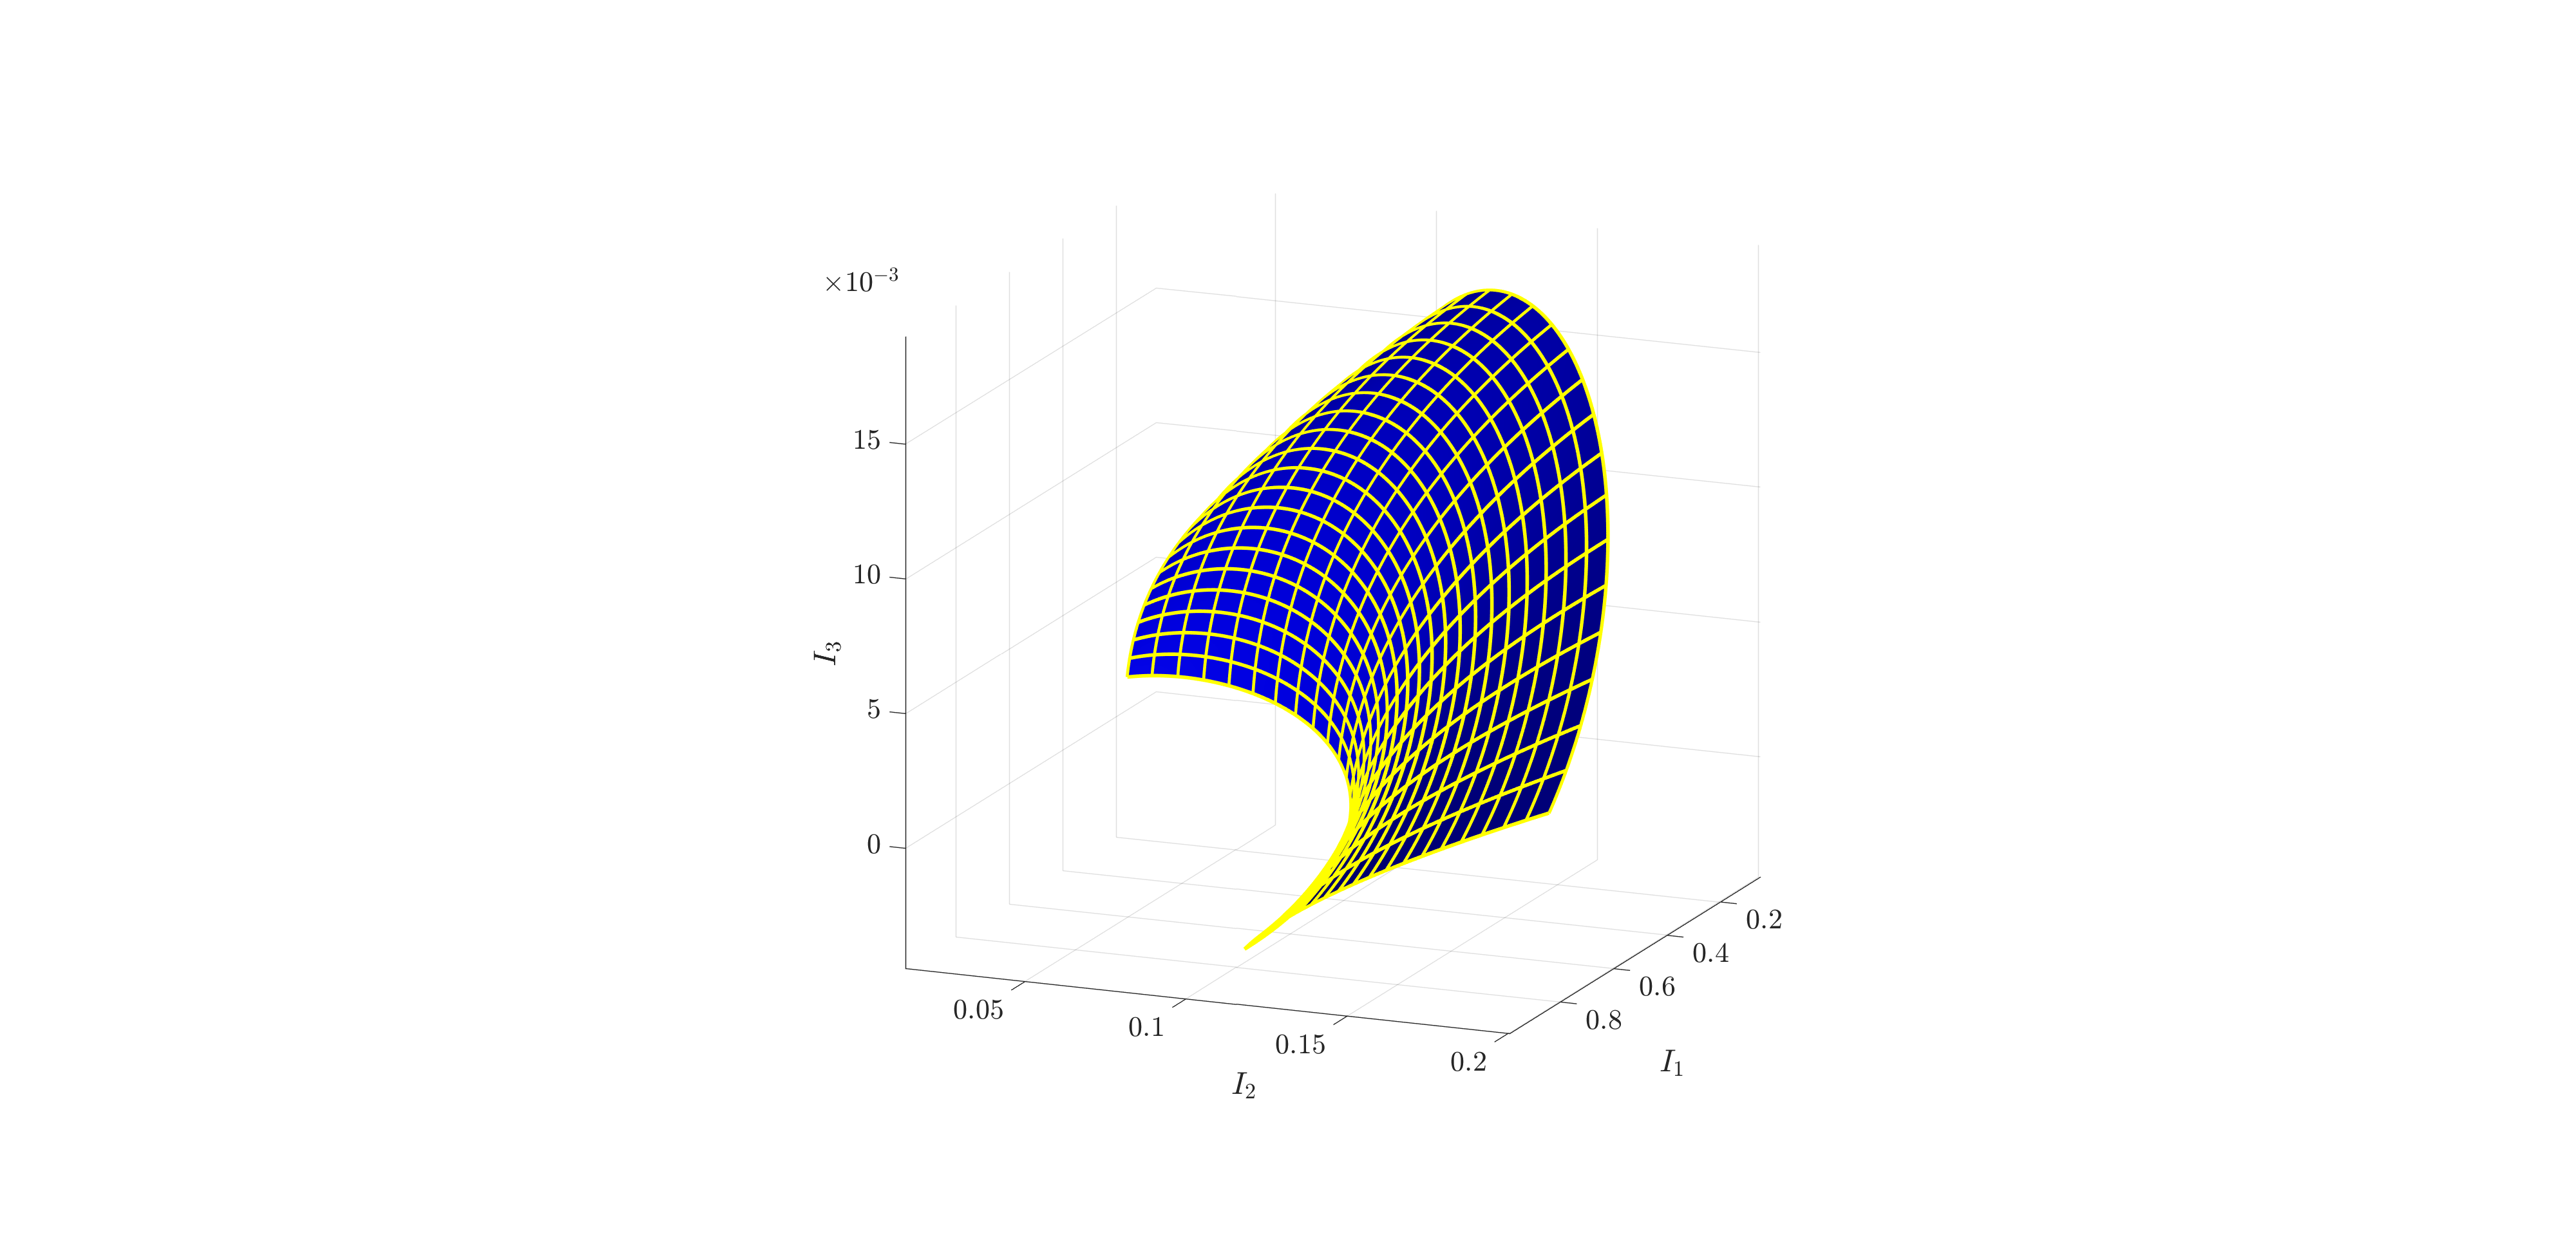
\includegraphics[width=12cm]{../images/SE2Transform_signature}
	\caption{SE(2) signature}
\end{figure}
\begin{figure}
	\includegraphics[width=12cm]{../images/E2Transform_signature}
	\caption{E(2) signature}
\end{figure}
\begin{figure}
	\includegraphics[width=12cm]{../images/SA2Transform_signature}
	\caption{SA(2) signature}
\end{figure}
\begin{figure}
	\includegraphics[width=12cm]{../images/A2Transform_signature}
	\caption{A(2) signature}
\end{figure}

\subsection{Hat tip to practicality: smoothing for E(2) and subgroups thereof}
Allows these groups to be used on real (i.e. not particularly
differentiable) images

\subsection{colour}

\section{Discussion and Conclusion or whatever}
Why are we using invariants? 
This idea is extremely local, can global information be better utilised?
Relation to using more computationally
tractable e.g. SA(2) not E(2)
Comparison with other invariant forms - e.g. Fourier, integral, etc.

\subsection{Future work}
Can we do better with the weights?
Can we do better with derivatives?
Projection onto Riemann sphere?
Noise. Ugh.

\begin{thebibliography}{99}
\bibitem{bessel} A. Bessel, Ueber die Invarianten der einfachsten Systeme simultaner bin\"arer Formen, Math. Ann. 1 (1869) 173--194.
\bibitem{draisma} M. I. P. Draisma, {\em Invariants of binary forms}, PhD thesis, Basel, 2014.
\end{thebibliography}
\end{document}
